%   Filename    : chapter_4.tex 


\chapter{Preliminary Results/System Prototype}
This chapter presents the preliminary results between the comparison of trained machine learning models: Logistic Regression, Random Forest,  Decision Trees, Support Vector Machine (SVM), and k-nearest Neighbors (KNN).  This chapter will also present the model evaluation and the comparison of model performance. 

\section{Data Summary}
\subsection{Dataset Overview}

\subsection{Preprocessing Results}

\section{Hyperparameter Optimization}

\begin{table}[H]
	\centering
	\resizebox{\linewidth}{!}{ 
		\begin{tabular}{lcc}
			\hline
			\textbf{Model} & \textbf{Best Parameters} & \textbf{Score}  \\ \hline
			Logistic Regression & \{'classifier\_\_C': 5\} & 0.744654  \\
			Decision Tree       & \{'criterion': 'gini', 'max\_depth': 10\} & 0.986164  \\
			Random Forest       & \{'n\_estimators': 50\} & 0.991195  \\
			SVM                 & \{'classifier\_\_C': 20, 'classifier\_\_kernel': 'rbf'\} & 0.862893  \\
			KNN                 & \{'classifier\_\_metric': 'manhattan', 'classifier\_\_n\_neighbors': 9, 'classifier\_\_weights': 'distance'\} & 0.991195  \\ \hline
		\end{tabular}
	}
	\caption{Hyperparameter Optimization}
	\label{tab:hyperparameter-optimization}
\end{table}


\section{Tuned Classifier Comparison}

\begin{table}[H]
	\centering
	\resizebox{\linewidth}{!}{ 
		\begin{tabular}{lcc}
			\hline
			\textbf{Model} & \textbf{Balanced Accuracy (\%)} & \textbf{Training Time (s)}  \\ \hline
			Logistic Regression & 74.35 & 3.07  \\
			Decision Tree       & 95.44 & 0.16  \\
			Random Forest       & 98.73 & 1.29  \\
			SVM                 & 74.64 & 0.12  \\
			KNN                 & 83.05 & 0.15  \\ \hline
		\end{tabular}
	}
	\caption{Tuned Classifier Comparison}
	\label{tab:tuned-classifier-comparison}
\end{table}



\section{Comparison of Model Performance}

To evaluate the performance of the different models used, the effectiveness of the models was evaluated and compared in predicting the sex of the \textit{T. granosa} based on morphological traits. The use of performance metrics such as accuracy, precision, recall, and F1-score is used to evaluate the performance of the different models. By analyzing the performance metrics, the researchers can identify the most effective and best model for the classification of male and female \textit{T. granosa}. 


\begin{table}[H]
	\centering
	\resizebox{\linewidth}{!}{ 
		\begin{tabular}{lcccc}
			\hline
			\textbf{Model} & \textbf{Ave Accuracy (\%)} & \textbf{Ave Precision (\%)} & \textbf{Ave Recall (\%)} & \textbf{Ave F1-score (\%)} \\ \hline
			Logistic Regression & 78.86 & 74.96 & 74.86 & 74.55 \\
			Decision Tree       & 98.11 & 98.22 & 98.11 & 98.12 \\
			Random Forest       & 98.68 & 98.74 & 98.68 & 98.68 \\
			SVM                 & 87.34 & 87.79 & 87.34 & 87.22 \\
			KNN                 & 99.43 & 99.45 & 99.43 & 99.43 \\ \hline
		\end{tabular}
	}
	\caption{Model Performance Comparison}
	\label{tab:model-performance}
\end{table}

Table ~\ref{tab:model-performance} presents the comparison results of machine learning models on the morphological traits of the combined  male and female \textit{T. granosa} datasets. The results indicate that all models demonstrated high performance in predicting male and female, with the F1-score ranging between 74-99\%. The KNN model achieved the highest accuracy (99.43\%), precision (99.45\%), recall (99.43\%) and F1-score (99.43\%), followed by random forest, decision tree, and SVM, respectively. However, the logistic regression was the worst classifier having an accuracy of (74.86\%), precision (74.96\%), recall (74.86\%) and (74.55\%) F1-score. Overall, the results seen in this comparison highlight that machine learning models are highly effective in predicting sex identification of \textit{T. granosa} based on their morphological features. With KNN being the best model, it suggests that non-parametric data and pattern recognition (H. Benhar, 2020) is well suited for this dataset. 

\section{Feature Importance Analysis}
After processing the dataset and splitting it into training and testing sets, the models are trained and their important features are computed. Feature analysis helps in identifying which morphological features contribute most in classifying male and female \textit{T. granosa}. The study uses models such as decision trees, and random forests to generate the scores. The models explore a wide range of features and then produce a score that reflects the feature’s importance in predicting the variable (Anitha \& Neelakandan, 2024).  

\begin{figure}[!htbp]
	\centering
	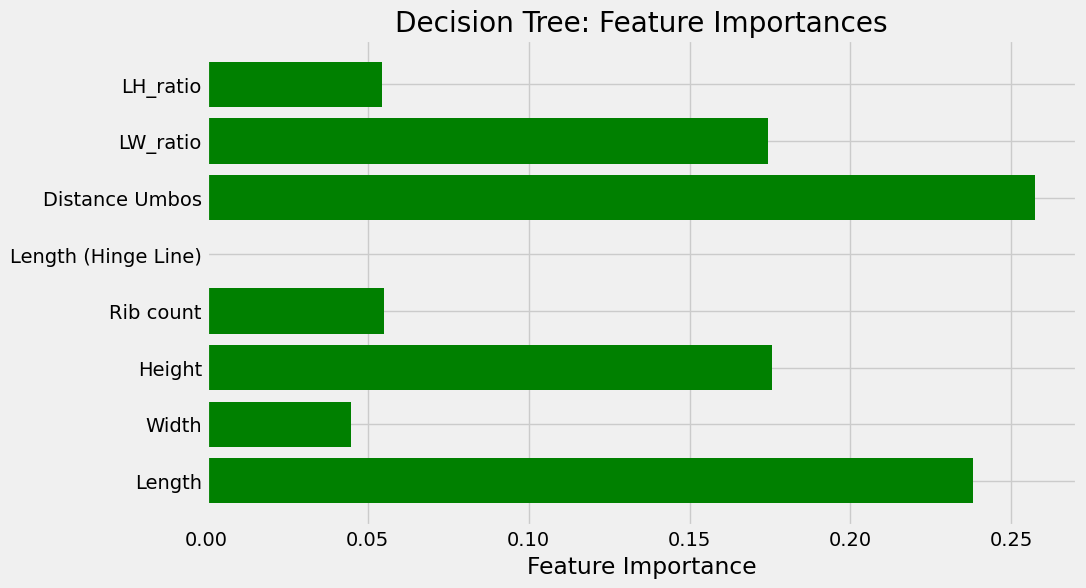
\includegraphics[width=0.8\textwidth]{figures/decision-trees.png}
	\caption{Feature Importance of Decision Trees}
	\label{fig:decision-trees}
\end{figure}

\begin{figure}[!htbp]
	\centering
	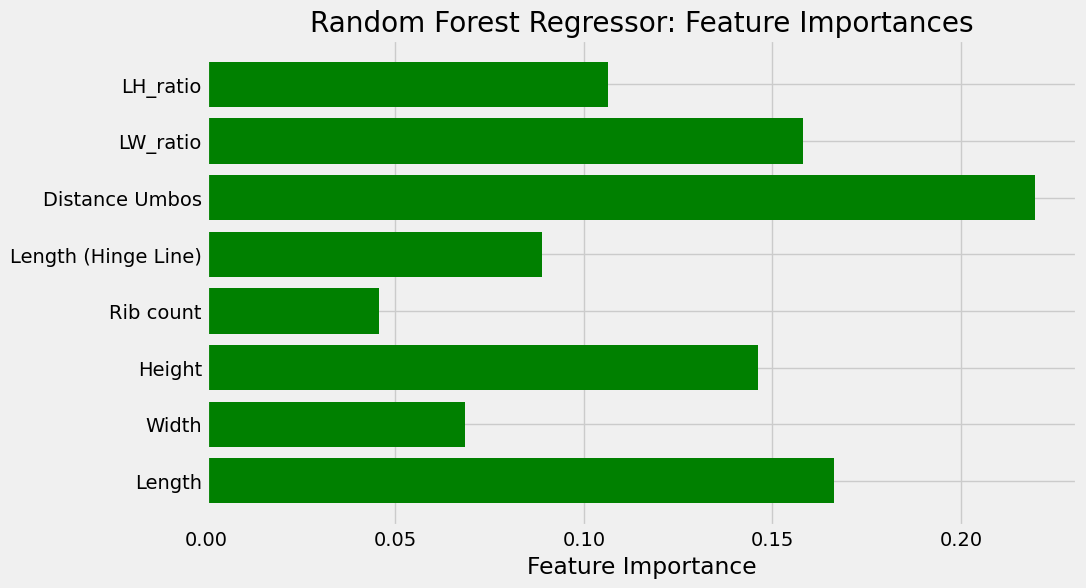
\includegraphics[width=0.8\textwidth]{figures/random-forest.png}
	\caption{Feature Importance of Random Forest}
	\label{fig:random-forest}
\end{figure}

To determine the important features that contribute to the classification of sex in \textit{T. granosa}, two machine learning models, decision trees, and random forest were compared based on the importance of the features. The results in figures ~\ref{fig:decision-trees} and ~\ref{fig:random-forest} indicates variations in feature importance between two models, however certain features such as distance of the umbos, LW\_ratio, length, and height consistently emerge as influential predictors. Hence, this analysis allowed the researchers to identify which features were most predictive that can improve the model’s performance. 

